\documentclass[10pt,notes]{beamer}
\usepackage{tcolorbox}

\usepackage{biblatex}
\bibliography{references.bib}

\usecolortheme{whale}
\useinnertheme{rounded}
\useoutertheme{infolines}

\linespread{1.4}\selectfont
\beamertemplatenavigationsymbolsempty
\setbeamerfont{note title}{size=\tiny}
\setbeamertemplate{footline}[frame number]
\setbeamertemplate{itemize item}[triangle]
\setbeamertemplate{itemize subitem}[circle]
\setbeamertemplate{itemize subsubitem}[square]

\setbeamertemplate{headline}
{
  \leavevmode%
  \hbox{%
  \begin{beamercolorbox}[wd=.5\paperwidth,ht=2.5ex,dp=1.5ex,right,rightskip=1em]{section in head/foot}%
    \usebeamerfont{subsection in head/foot}\hspace*{2ex}\insertshorttitle
  \end{beamercolorbox}%
  \begin{beamercolorbox}[wd=.5\paperwidth,ht=2.5ex,dp=1.5ex,left,leftskip=1em]{subsection in head/foot}%
    \usebeamerfont{section in head/foot}\insertsectionhead\hspace*{2ex}
  \end{beamercolorbox}}%
  \vskip0pt%
}

\setbeamertemplate{frametitle}{%
    \nointerlineskip%
    \begin{beamercolorbox}[wd=\paperwidth,ht=3.0ex,dp=1.6ex]{frametitle}
        \hspace*{1.5ex}\insertframetitle%
    \end{beamercolorbox}%
}

\makeatletter
\setbeamertemplate{footline}
{
  \leavevmode%
  \hbox{%
  \begin{beamercolorbox}[wd=.925\paperwidth,ht=2.5ex,dp=1ex,center]{author in head/foot}%
    \usebeamerfont{author in head/foot}\insertshortauthor
  \end{beamercolorbox}%
  \begin{beamercolorbox}[wd=.075\paperwidth,ht=2.5ex,dp=1ex,right]{date in head/foot}%
    \insertframenumber{} / \inserttotalframenumber\hspace*{2ex} 
  \end{beamercolorbox}}%
  \vskip0pt%
}
\makeatother

\makeatletter
\defbeamertemplate*{note page}{infolines}
{%
  {%
    \usebeamerfont{note title}\usebeamercolor[fg]{note title}%
    \ifbeamercolorempty[bg]{note title}{}{%
      \insertvrule{.0325\paperheight}{note title.bg}%
      \vskip-.0325\paperheight%
      \nointerlineskip%
    }%
    \nointerlineskip
    \leavevmode
    \vbox to .0325\paperheight{\vfil
        \begin{minipage}[t]{.5\linewidth}%
            \hfill\insertshorttitle\hspace*{2ex}
        \end{minipage}%
        \begin{minipage}[t]{.5\linewidth}%
            \hspace*{2ex}\insertsectionhead\hfill
        \end{minipage}%
    \vfil}%
  }%
  
  \ifbeamercolorempty[bg]{note page}{}{%
    \nointerlineskip%
    \insertvrule{.965\paperheight}{note page.bg}%
    \vskip-.965\paperheight%
  }%
  \vskip.25em
  \nointerlineskip
  \insertnote
}
\makeatother
\setbeamertemplate{note page}[infolines]

\title{Open Queueing Networks}
\author{Himanshu Singh \and Vikaskumar Kalsariya \and Aditya Kulkarni \and Kiran Gullapalli \and Keshava V}
\date{March 2, 2024}

\begin{document}

\begin{frame}
    \titlepage
\end{frame}

\begin{frame}
    \tableofcontents
\end{frame}

\section{Introduction}

\begin{frame}
    \frametitle{Queueing Networks}
    \begin{itemize}
        \item A queueing network is a connected directed graph, whose nodes represent servers (each with their own queue), and edges between nodes represent channels through which jobs can be routed.
    \end{itemize}
    \begin{figure}
        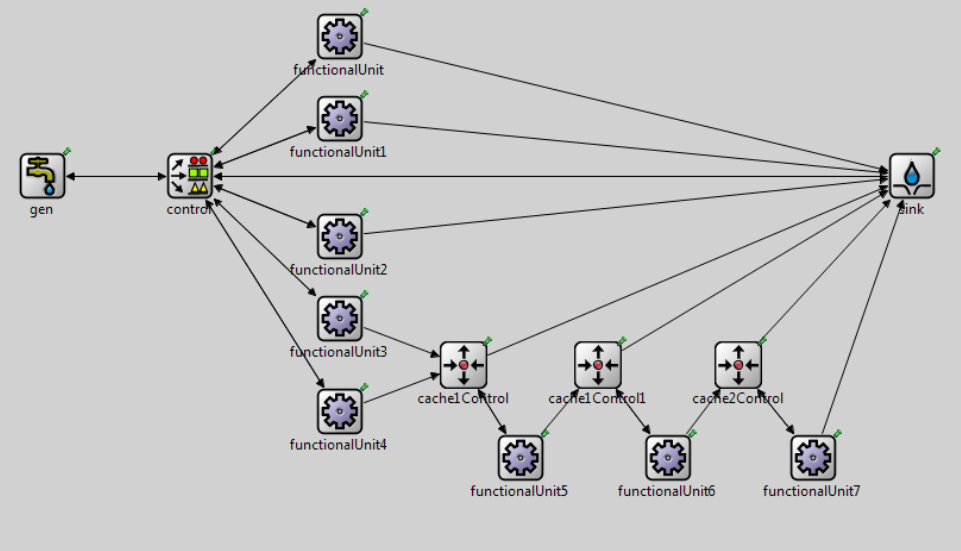
\includegraphics[width=0.6\linewidth]{images/ivy_bridge.png}
        \caption{Intel Ivy Bridge queue model \cite{damian}}
    \end{figure}
\end{frame}
    
\begin{frame}
    \frametitle{Open Networks}
    \begin{itemize}
        \item A network is said to be open if there is at least one edge for an `external' arrival, and from every node there is a path for an `external' departure.
    \end{itemize}
    \begin{figure}
        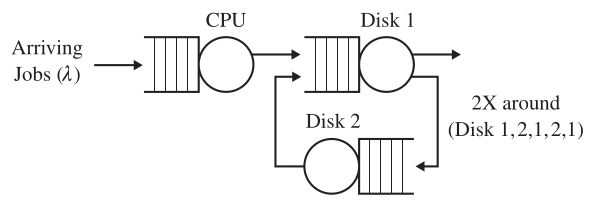
\includegraphics[width=0.55\linewidth]{images/open_network.png}
        \caption{An open queueing network}
    \end{figure}
\end{frame}

\begin{frame}
    \frametitle{Jackson Network}
    \begin{itemize}
        \item A general form of open network
            \begin{itemize}
                \item Unbounded queues, with FCFS service order
                \item External arrivals \(\sim\) Poisson(\(r_i\))
                \item Service rates \(\sim\) Exp(\(\mu_i\))
                \item Probabilistic routing - \(P_{ij}\)
                \item States: \((n_1, n_2, \ldots, n_k)\)
            \end{itemize}
    \end{itemize}
    \begin{figure}
        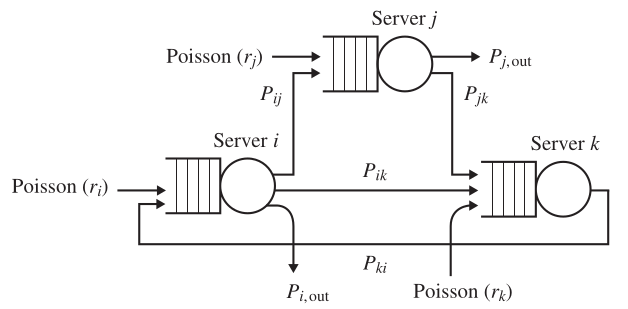
\includegraphics[width=0.55\linewidth]{images/jackson_network.png}
        \caption{A Jackson network}
    \end{figure}
\end{frame}

\begin{frame}
    \frametitle{Poisson Arrivals?}
        \begin{itemize}
            \item $\lambda_i = r_i + \sum_j \lambda_j P_{ji}$
            \item Consider a single server network with properties:
            \begin{itemize}
                \item Low arrival rate
                \item High service rate
                \item High \(P_{ii}\)
            \end{itemize}
        \end{itemize}
        \begin{figure}
            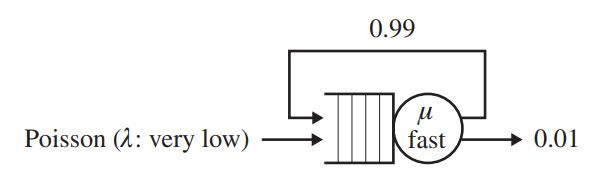
\includegraphics[width=0.65\linewidth]{images/independency_network.jpg}
        \end{figure}
        \begin{center} 
            Violates independent increment property!
        \end{center}

\end{frame}

\section{Solving the Jackson Network}

\begin{frame}
    \frametitle{Balance Equations}
    \begin{itemize}
        \item Rate of jobs leaving the state = Rate of jobs entering the state.
    \end{itemize}
    \begin{center} 
        \[\pi_{n_1,n_2,\ldots,n_k} \cdot \left[ \sum_{i=1}^{k} r_i + \sum_{i=1}^{k} \mu_i (1 - P_{ii})  \right] =\]
        \begin{equation}
            \linespread{1.6}
            \begin{aligned}
                \notag
                &\underbrace{\sum_{i=1}^{k} \pi_{n_1,\ldots,n_i - 1,\ldots,n_k} \cdot r_i}_{\text{outside arrival}}
                + \underbrace{\sum_{i=1}^{k} \pi_{n_1,\ldots,n_i + 1,\ldots,n_k} \cdot \mu_i P_{i,\text{out}}}_{\text{departure to outside}} \\
                &+ \underbrace{\sum_{i=1}^{k} \sum_{j \neq i} \pi_{n_1,\ldots,n_i - 1,\ldots,n_j + 1,\ldots,n_k} \cdot \mu_j P_{ji}}_{\text{internal transition from server } j \text{ to server } i, \ j \neq i}
            \end{aligned}
        \end{equation}

        
    \end{center}
    

\end{frame}

\begin{frame}
    \frametitle{Balance Equations (Contd.)}
    \begin{itemize}
        \item In general, very hard to solve.
        \item Local Balance Approach
        \begin{itemize}
            \item Break both sides of the equation into $k+1$ matching components and equate each component.
            \item Define $A$ = Rate of leaving state due to an external arrival.
            \item Define $A'$ = Rate of entering state due to an external departure.
            \item Define $B_i$ = Rate of leaving state due to a depature from server $i$.
            \item Define $B_i'$ = Rate of entering state due to an arrival at server $i$.
        \end{itemize}
    \end{itemize}
\end{frame}

\begin{frame}
    \frametitle{Balance Equations (Contd.)}
    \begin{itemize}
        \item Solving A = A'
            $$\sum_{i=1}^{k} \pi_{n_1,\ldots,n_i,\ldots,n_k} \cdot r_i = \sum_{i=1}^{k} \pi_{n_1,\ldots,n_i+1,\ldots,n_k} \cdot \mu_i P_{i,\text{out}}$$
        \item Can we make a guess for \(\pi_{n_1,\ldots,n_k}\) such that it satisfies the above equality?
        \item Observe that \(\pi_{n_1,\ldots,n_i,\ldots,n_k}\) term in $A$ and the \(\pi_{n_1,\ldots,n_i+1,\ldots,n_k}\) term in $A'$ only differ in $n_i$.
        \item Let us assume that
            $$\pi_{n_1,\ldots,n_i,\ldots,n_k} \cdot c_i = \pi_{n_1,\ldots,n_i+1,\ldots,n_k}$$
        \item Substituting, we get
            $$\sum_{i=1}^{k} r_i = \sum_{i=1}^{k} (c_i \cdot \mu_i) P_{i,\text{out}}$$
    \end{itemize}
\end{frame}

\begin{frame}
    \frametitle{Balance Equations (Contd.)}
    \begin{itemize}
        \item If we further assume $c_i \cdot \mu_i = \lambda_i$, we get $$\sum_{i=1}^{k} r_i = \sum_{i=1}^{k} \lambda_i P_{i,\text{out}}$$
        \item By our assumption, $c_i = \dfrac{\lambda_i}{\mu_i} = \rho_i$. Substituting this we get
            $$\pi_{n_1}, \ldots, \pi_{n_i}, \ldots, \pi_{n_k} \cdot \rho_i = \pi_{n_1}, \ldots, \pi_{n_i+1}, \ldots, \pi_{n_k}$$
        \item Repeating the argument yields the following equation
            $$\pi_{n_1}, \ldots, \pi_{n_k} = C \rho_{1}^{n_1} \ldots \rho_{k}^{n_k}$$
    \end{itemize}
\end{frame}

\begin{frame}
    \frametitle{Balance Equations (Contd.)}
    \begin{itemize}
        \item We still need to check if our assumption yields a valid solution to $B_i = B_i'$
    \end{itemize}
    \begin{align*}
        B_i &= B'_i \\
        C \rho_1^{n_1} \rho_2^{n_2} \cdots \rho_k^{n_k} \mu_i (1 - P_{ii}) &= \sum_{j \neq i} C \rho_1^{n_1} \rho_2^{n_2} \cdots \rho_k^{n_k} \left( \frac{\rho_j}{\rho_i} \right) \mu_j P_{ji} \\
        &\phantom{=} + C \rho_1^{n_1} \rho_2^{n_2} \cdots \rho_k^{n_k} \left( \frac{1}{\rho_i} \right) r_i \\
        \mu_i (1 - P_{ii}) &= \sum_{j \neq i} \frac{\rho_j \mu_j P_{ji}}{\rho_i} + \frac{r_i}{\rho_i} \\
        \rho_i \mu_i (1 - P_{ii}) &= \sum_{j \neq i} \rho_j \mu_j P_{ji} + r_i \\
        \lambda_i (1 - P_{ii}) &= \sum_{j \neq i} \lambda_j P_{ji} + r_i
    \end{align*}

\end{frame}

\begin{frame}
    \frametitle{Balance Equations (Contd.)}
    \begin{itemize}
        \item Lastly, we need to find the normalizing constant $C$.
            $$\sum_{n_1,\ldots,n_k} \pi_{n_1,\ldots,n_k} = 1$$
            $$C \sum_{n_1,\ldots,n_k} \rho_1^{n_1} \cdots \rho_k^{n_k} = 1$$
            $$C \left( \sum_{n_1} \rho_1^{n_1} \right) \left( \sum_{n_2} \rho_2^{n_2} \right) \cdots \left( \sum_{n_k} \rho_k^{n_k} \right) = 1$$
            $$C \left( \frac{1}{1 - \rho_1} \right) \left( \frac{1}{1 - \rho_2} \right) \cdots \left( \frac{1}{1 - \rho_k} \right) = 1$$
            $$C = (1 - \rho_1) (1 - \rho_2) \cdots (1 - \rho_k).$$
    \end{itemize}
    \begin{tcolorbox}
        \centering $\pi_{n_1,\ldots,n_k} = \rho_1^{n_1} (1 - \rho_1) \rho_2^{n_2} (1 - \rho_2) \cdots \rho_k^{n_k} (1 - \rho_k)$
    \end{tcolorbox}
\end{frame}

\begin{frame}
    \frametitle{Balance Equations (Contd.)}
    \begin{itemize}
        \item What about the jobs at a given server?
            \begin{align*}
                P\{n_1 \text{ jobs at server } 1\} &= \sum_{n_2,\ldots,n_k} \pi_{n_1,\ldots,n_k} \\
                &= \sum_{n_2,\ldots,n_k} \rho_1^{n_1} (1 - \rho_1) \rho_2^{n_2} (1 - \rho_2) \cdots \rho_k^{n_k} (1 - \rho_k) \\
                &= \rho_1^{n_1} (1 - \rho_1)
            \end{align*}
        
        \begin{tcolorbox}
            \centering $P\{n_i \text{ jobs at server } i\} = \rho_i^{n_i} (1 - \rho_i)$
        \end{tcolorbox}
        \item Thus, all servers behave like M/M/1 queues in terms of their stationary queue length distributions, even though their arrival processes are not necessarily Poisson.
    \end{itemize}
\end{frame}

\begin{frame}
    \frametitle{Summary}
    \begin{tcolorbox}
        \centering $\lambda_i = r_i + \sum_j \lambda_j P_{ji}$
    \end{tcolorbox}
    \begin{tcolorbox}
        \centering $\rho_i = \frac{\lambda_i}{\mu_i}$
    \end{tcolorbox}
    \begin{tcolorbox}
        \centering $\pi_{n_1,\ldots,n_k} = \rho_1^{n_1} (1 - \rho_1) \rho_2^{n_2} (1 - \rho_2) \cdots \rho_k^{n_k} (1 - \rho_k)$
    \end{tcolorbox}
    \begin{tcolorbox}
        \centering $P\{n_i \text{ jobs at server } i\} = \rho_i^{n_i} (1 - \rho_i)$
    \end{tcolorbox}
    \begin{tcolorbox}
        \centering $E\{N_i\} = \dfrac{\rho_i}{1 - \rho_i}$
    \end{tcolorbox}
\end{frame}

\section{Simulation}

\begin{frame}
    \frametitle{Case 1}
    \begin{figure}
        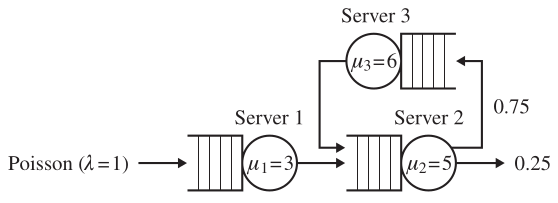
\includegraphics[width=0.75\linewidth]{images/case1.png}
    \end{figure}
\end{frame}

\begin{frame}
    \frametitle{Case 1}
    \begin{itemize}
        \item $\lambda_1 = 1$ \\
            $\lambda_2 = \lambda_1 + \lambda_3$ \\
            $\lambda_3 = 0.75\lambda_2$
        \item $\lambda_1 = 1, \lambda_2 = 4, \lambda_3 = 3$
        \item $\rho_1 = \frac{1}{3}, \rho_2 = \frac{4}{5}, \rho_3 = \frac{1}{2}$
        \item $E[N_1] = \frac{1}{2}, E[N_2] = 4, E[N_3] = 1$
    \end{itemize}
\end{frame}

\begin{frame}
    \frametitle{Case 2}
    \begin{figure}
        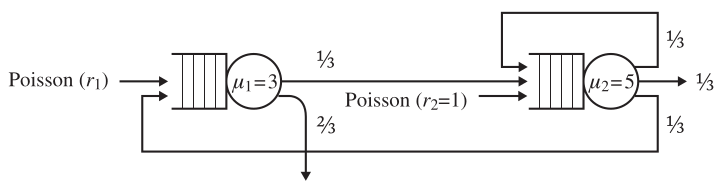
\includegraphics[width=0.7\linewidth]{images/case2.png}
    \end{figure}
\end{frame}

\begin{frame}
    \frametitle{Case 2}
    \begin{itemize}
        \item $\lambda_1 = r_1 + \frac{1}{3}\lambda_2$ \\
            $\lambda_2 = 1 + \frac{1}{3}\lambda_1 + \frac{1}{3}\lambda_2$ \\
        \item $\lambda_1 = \frac{6r_1 + 3}{5}, \lambda_2 = \frac{3r_1 + 9}{5}$
        \item $\rho_1 = \frac{2r_1 + 1}{5}, \rho_2 = \frac{3r_1 + 9}{25}$
        \item For $\rho_1 < 1$, $r_1 < 2$. Let $r_1 = 1.5$.
        \item $\lambda_1 = 2.4, \lambda_2 = 2.7$
        \item $\rho_1 = 0.8, \rho_2 = 0.34$
        \item $E[N_1] = 4, E[N_2] = 1.17$
    \end{itemize}
\end{frame}

\begin{frame}
    \frametitle{Case 3}
    \begin{figure}
        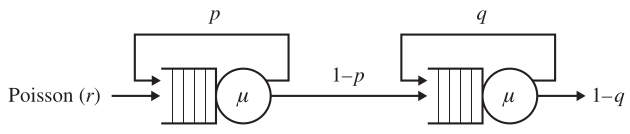
\includegraphics[width=0.75\linewidth]{images/case3.png}
    \end{figure}
\end{frame}

\begin{frame}
    \frametitle{Case 3}
    \begin{itemize}
        \item $\lambda_1 = r + p\lambda_1$ \\
            $\lambda_2 = (1 - p)\lambda_1 + q\lambda_2$ \\
        \item $\lambda_1 = \frac{r}{1 - p}, \lambda_2 = \frac{r}{1 - q}$
        \item $\rho_1 = \frac{r}{\mu(1 - p)}, \rho_2 = \frac{r}{\mu(1 - q)}$
        \item $E[N_1] = \frac{r}{\mu(1 - p) - r}, E[N_2] = \frac{r}{\mu(1 - q) - r}$
        \item Let $r = 0.5, \mu = 3, p = 0.1, q = 0.2$.
        \item $\lambda_1 = \frac{5}{9}, \lambda_2 = \frac{5}{8}$
        \item $\rho_1 = \frac{5}{27}, \rho_2 = \frac{5}{24}$
        \item $E[N_1] = 0.23, E[N_2] = 0.26$
    \end{itemize}
\end{frame}

\section{References}

\begin{frame}
    \frametitle{References}
    \nocite{*}
    \printbibliography
\end{frame}

\end{document}
